\bichapter{试验材料和方法}{Material and methods}

\bisection{实验试剂与仪器}{Chemical reagents and instrument analyses}

\subsection{实验试剂}

本文研究主要用到的实验试剂如\cref{tab1}

\begin{table}[h]
	\centering
	\bicaption{主要实验试剂}{Main experimental reagents}
	\label{tab1}
	\begin{tabular}{@{}cccc@{}}
        \toprule
		试剂名称&分子式&纯度&生产厂家\\
        \midrule
		海藻酸钠&X&AR&天津市福晨化学试剂厂\\
		硫化钠&$\mathrm{Na_2S}$&AR&天津市福晨化学试剂厂\\
		硼氢化钠&$\mathrm{NaBH}$&AR&天津市福晨化学试剂厂\\
		硫酸亚铁&$\mathrm{FeSO_4\cdot7H_2O}$&AR&天津市福晨化学试剂厂\\
		盐酸&$\mathrm{HCl}$&AR&天津市福晨化学试剂厂\\
        氢氧化钠&$\mathrm{NaOH}$&AR&天津市福晨化学试剂厂\\
        盐酸羟胺&$\mathrm{HONH_3Cl}$&AR&天津市福晨化学试剂厂\\
        邻菲啰啉&$\mathrm{C_12H_8N_2H_2O}$&AR&天津市福晨化学试剂厂\\
        氮气&$\mathrm{N_2}$&LP&北京海瑞通达气体科技有限公式\\
        \bottomrule
	\end{tabular}
\end{table}

\section{主要试验仪器}

试验过程中主要使用到的仪器和设备见\cref{tab2}

\begin{table}[h]
	\centering
	\bicaption{主要实验试剂}{Main experimental reagents}
	\label{tab2}
	\begin{tabular}{@{}ccc@{}}\toprule
		仪器名称&规格型号&生产厂家\\\midrule
		精密定时电动搅拌器&JJ-1&北京市中兴伟业仪器有限公司\\
        超声波细胞粉碎机&BILON-650Y&上海比朗仪器制造有限公司\\
		冷冻干燥机&FD-1A-50&上海比朗仪器制造有限公司\\
		流量型蠕动泵&BT100-1L&保定兰格恒流泵有限公司\\
		紫外可见分光光度计&2082S UV/VIS&上海尤尼柯仪器有限公司\\
		电子天平&JA2003&上海恒平科学仪器有限公司\\
        Zeta电位及粒度分析仪&90Plus Zeta&美国布鲁克海文仪器公司\\
        真空干燥箱&DZ-2AII&天津市泰斯特仪器有限公司\\\bottomrule
	\end{tabular}
\end{table}

\bisection{实验装置}{}

\bisection{分析方法}{Analytical method}

\subsection{海藻酸钠改性硫化型纳米铁的制备}\label{material}

用于制备SA-S-NZVI的海藻酸钠和硫化钠购自天津市福晨化学试剂厂。超纯水(SIM-T30UV,北京飞翔赛思科技有限公司)在反应前通过氮气(北京顺驰东环干冰经营中心)进行脱氧。实验的所有试剂均为分析纯,所有溶液和稀释液均在超纯水中制备。

采用表面腐蚀法制备S-nZVI,$\mathrm{S^{2-}}$水解产生$\mathrm{HS^-}$和$\mathrm{H_2S}$对nZVI具有腐蚀作用,生成的$\mathrm{Fe^{2+}}$与$\mathrm S^{2-}$结合,在nZVI表面生成FeS\cite{ ISI:000382805800072}。使用液相还原法制备NZVI\cite{2020The,LIU2019124193},将2.48 g$\mathrm{FeSO_4\cdot 7H_2O}$ 溶解于350 ml超纯水中。取0.68 g$\mathrm{NaBH_4}$溶于150 ml超纯水后逐滴加入到上述溶液中。同时用电动搅拌机(JJ-1,北京市中兴伟业仪器有限公司)以600 $\mathrm{r\cdot min^{-1}}$的转速搅拌,反应完成后继续搅拌15 min,反应式如\cref{eq1}。将混合液过滤,收集的固体颗粒用去离子水冲洗2次,无水乙醇冲洗1次,将其干燥后密封置于冰箱中保存。配置1 g/L的NZVI悬浊液,超声10 min,向其中加入0.32 g $\mathrm{{Na}_2S}$,使用电动搅拌机搅拌2 h,获得S/Fe比(摩尔比)为0.15的S-nZVI。其反应式如\cref{e16}所示\cite{ ISI:000355774400014}。

\begin{equation}\label{eq1}
    \mathrm{{Fe}^{2+}+2{BH}_4^-+4H_2O}\rightarrow \mathrm{2{Fe}^0\left(s\right)+{B\left(OH\right)}_4^-+4H^+}\mathrm{+2H_2\left(g\right)}
\end{equation}
\begin{equation}
    \mathrm{{Na}_2S+H_2O\rightarrow2{Na}^++{HS}^-+{OH}^-}
\end{equation}
\begin{equation}
    \mathrm{{Fe}^{2+}+2{HS}^-\rightarrow FeS(s)+H_2S}
\end{equation}
\begin{equation}\label{e16}
    \mathrm{S^{2-}+{Fe}^{2+}\rightarrow FeS(s)}
\end{equation}

将0.5 g的S-NZVI颗粒分别分散在不同浓度的海藻酸钠的水溶液中(0.0、0.1、0.2、0.3 wt\%),超声处理30 min。然后27500 rpm转速离心80 min,倒去上清液,用超纯水清洗数次后干燥备用。样品依次记为S-NZVI,0.1\%SA-S-NZVI,0.2\%SA-S-NZVI和0.3\%SA-S-NZVI。

\subsection{材料的表征}

将S-NZVI悬浮于0.1 mM的NaCl溶液中,使用NaOH或HCl调整溶液pH,使用超声细胞粉碎机中超声30 min。使用Zeta电位及粒度分析仪(90Plus Zeta, Brookhaven Instruments Corporation)测定不同pH在3到10范围内S-NZVI的电泳迁移率($u_e$)。S-NZVI的$\zeta$电位由Smoluchowski方程计算:$\zeta=\eta u_\mathrm{e}/\varepsilon$。其中$\eta$为水粘度,$\varepsilon$为水的介电常数。将\cref{material}制备完成的4种样品分别悬浮于不同离子强度的NaCl溶液中(5.0,10.0,20.0,40.0,60.0,80.0 mM),调节溶液pH为8,测定样品的电泳迁移率。

使用0.1 mM NaCl溶液将\cref{material}制备完成的4种样品配置成1.0 g/L的悬浮液,调整溶液pH=8放入石英比色皿,使用紫外分光光度计(2082S UV/VIS,Unico Instrument Corporation)在508 nm波长下测定不同时刻对铁的吸光度,扫描时间4000 s,扫描间隔30 s。
    
利用Zeta电位及粒度分析仪(90Plus Zeta, Brookhaven Instruments Corporation)的动态光散射(DLS)模块测定SA-S-NZVI纳米颗粒的颗粒尺寸($a_\mathrm{h}$)。将上述样品配置成0.015 g/L的悬浮液,使用NaOH或HCl调整溶液pH=8,于氮气气氛超声30 min后立即测量。散射光由光电探测器以$90^\circ$散射角检测,每次检测60 s。根据瑞利近似,散射光强度与粒径的六次方正相关,因此强度分布对粒径特别敏感,不适用与宽分布样品(图 S1)。为了有效确定团聚颗粒的粒径分布,对比了DLS的强度平均(by intensity)数据和数量平均(by number)数据。本文选择使用水力粒径的数量平均值以表征颗粒的尺寸分布。


\subsection{附着效率计算}

通过计算初始团聚速率常数$k$和附着效率$(\alpha)$来表征SA-nZVI的团聚动力学。团聚行为刚开始时,水力半径$a_\mathrm{h}$与时间$t$呈线性关系。因此,初始团聚速率常数($k$)可以通过对$a_\mathrm{h}(t)$随t的变化量进行线性最小二乘回归分析得到。该回归分析通常在从$t = 0$到$a_\mathrm{h}(t)$的值达到$1.25a(0)$的时间范围内进行\cite{ChenElimelech-762}。由\cref{1-20}计算不同离子强度下颗粒的初始团聚速率\cite{ChenMylon-760}:

\begin{equation}\label{1-20}
    k\propto\frac{1}{N_0}\left(\frac{\mathrm{d}a_\mathrm{h}(t)}{\mathrm{d}t}\right)_{t\rightarrow0}
\end{equation}

其中,$N_0$为纳米颗粒悬浊液的初始浓度。附着效率$\alpha_{\mathrm {pp}}$反映了颗粒之间发生有效碰撞的几率。它被定义为反应受限团聚(并非所有的碰撞都是有效的,团聚的发生需要颗粒的能量超过反应势垒,因此碰撞效率($\alpha_\mathrm{pp}<1$)与扩散受限团聚(聚集的发生由布朗运动引起,只要颗粒发生接触,就会形成更大的团簇,即碰撞效率($\alpha_\mathrm{pp}=1$)。导出的团聚速率之比\cite{doi:10.1021/la062072v}:

\begin{equation}\label{alpha_ppexp}
  \alpha_{\mathrm{pp}}=\frac{k}{k_{\mathrm{fast}}}=\frac{\frac{1}{N_0}\left(\frac{\mathrm{d}a_\mathrm{h}(t)}{\mathrm{d}t}\right)_{t\rightarrow0}}{\frac{1}{N_{0,\mathrm{fast}}}\left(\frac{\mathrm{d}a_\mathrm{h}(t)}{\mathrm{d}t}\right)_{t\rightarrow0,\mathrm{fast}}}
\end{equation}

其中,下标“fast”指扩散受限团聚。$k_{\mathrm{fast}}$取扩散限制团聚阶段下$k$的平均值。

\section{理论和模型计算}

\subsection{聚电解层厚度计算}

由于溶液中的阴阳离子和电荷可以透过包覆型S-NZVI表面,分布在吸附层内部,因此测量电泳迁移率结合Ohshima的软粒子理论来确定聚电解质吸附层的特性。Ohshima认为,软粒子周围的电势由吸附层内厚度为$d$的Donnan电势($\psi_\mathrm{DON}$)和吸附层与溶液边界的表面电势($\psi_\mathrm{0}$)组成\cite{2006315,OHSHIMA20152,Ohshima1995}(\cref{donnan})。结合Navier-Stokes方程计算吸附层的摩擦力,软粒子的电泳迁移率的表达式为\cite{Oshima1992}:

\begin{equation}\label{psidon}
    \psi _\mathrm{DON}=\frac{k_BT}{ze_0}\ln[\frac{ZN}{2zn}+\{(\frac{ZN}{2zn})^2+1\}^{1/2}]
\end{equation}
\begin{equation}\label{psi0}
    \psi_0=\psi_\mathrm{DON}-\frac{k_BT}{ze_0}\tanh\frac{ze_0\psi_\mathrm{DON}}{2k_BT}+\frac{4k_BT}{ze_0}\cdot e^{-\kappa_md}\cdot\tanh\frac{ze_0\zeta }{4k_BT}
\end{equation}
\begin{equation}
    \kappa=\sqrt{\frac{2nz^2e_0^2}{\varepsilon k_B T}}
\end{equation}
\begin{equation}
    \kappa_\mathrm{m}=\kappa\sqrt{\cosh(\frac{ze_0\psi_\mathrm{DON}}{k_BT})}
\end{equation}
\begin{align}\label{ue}
    u_\mathrm{e}=&\frac{\varepsilon}{\eta }\cdot\frac{\psi _0/\kappa _m+\psi _\mathrm{DON}/\lambda }{1/\kappa _m+1/\lambda }\cdot\frac{2}{3}\cdot[1+\frac{1}{2(1+d/a)^3}]\\ &+\frac{Ze_0N}{\eta \lambda ^2}+\frac{8\varepsilon k_BT}{\eta \lambda ze_0}\cdot\tanh \frac{ze_0\zeta}{4k_BT}\cdot\frac{e^{-\lambda d}/\lambda -e^{-\kappa _md}/\kappa _m}{1/\lambda ^2-1/\kappa _m^2}\nonumber
\end{align}

其中,$Z$为聚电解质电离基团的价态;$N(\mathrm{m^{-3}})$为包覆层中聚电解质的浓度;$z$为水相中电解质的价态(本文中使用NaCl,z取1);$n$为电解质的浓度;$e_0$为电子电荷;$k_\mathrm{B}$为玻尔兹曼常数;$\kappa_m$为有效徳拜常数;$a$、$d$分别为颗粒粒径和包覆层厚度;$\zeta$为裸S-NZVI的$\zeta$电位;$1/\lambda$为参数,其大小代表聚电解质层的软度,当$1/\lambda\rightarrow 0$时,包覆层为刚性,此时\cref{ue}等价于Smoluchowski方程。测定不同离子强度下裸S-NZVI和包覆型S-NZVI的电泳迁移率用于拟合\cref{psidon,psi0,ue}得到$N$、$\lambda$和$d$。

\begin{figure}
    \centering
    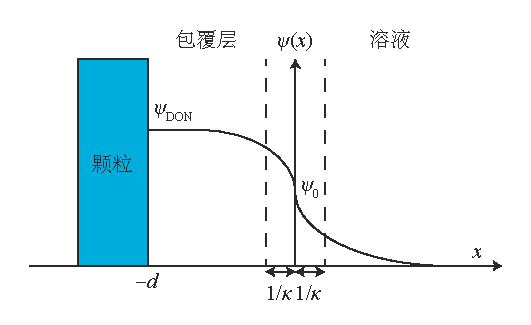
\includegraphics[width=12cm]{figs/Donnan-potential.pdf}
    \bicaption{软粒子表面的电势示意图}{Schematic diagram of the electric potential on the surface of a soft particle}\label{donnan}
\end{figure}

\subsection{碰撞频率的计算}

碰撞频率函数反映的是颗粒在分散体系中单位时间碰撞的次数。水环境中,粒子碰撞的机制主要为三种:布朗运动、流体剪切和差速沉降\cite{ThomasJudd-749}。采用Coalesced Fractal Sphere(CFS)模型\cite{LeeBonner-748}:(1)所有的絮凝体由单一类型的初级颗粒组成,这些初级颗粒是致密的球体。(2)所有絮凝体都具有固定的分形维数,且不受絮凝体粒径的影响。(3) 当两个絮凝体碰撞并结合时,新形成的絮凝体具有与碰撞前絮凝体相同的分形维数,新絮凝体的固体体积是碰撞前絮凝体的固体体积之和。布朗运动、流体剪切和差速沉降三种碰撞频率函数$\beta_{BR}$、$\beta_{SH}$、$\beta_{DS}$按下式计算\cite{LeeBonner-748}:
\begin{equation}\label{beta_br}
    \beta_{BR}(v_i,v_j)=\frac{2kT}{3\mu}(v_i^{1/D_F}+v_j^{1/D_F})(v_i^{-1/D_F}+v_j^{-1/D_F})
\end{equation}
\begin{equation}\label{beta_sh}
    \beta_{SH}(v_i,v_j)=\frac{G}{\pi}v_0^{1-3/D_F}{(v_i^{1/D_F}+v_j^{1/D_F})}^3
\end{equation}
当$D_F\in[2,3]$时
\begin{align}\label{beta_ds}
    \beta_{DS}(v_i,v_j)=&\frac{g}{12\mu}{(\frac{\pi}{6})}^{-1/3}[(\rho_0-\rho_w)/\rho_w]v_0^{1/3-1/D_F}\\ & \times(v_i^{1/D_F}+v_j^{1/D_F})^2\left|v_i^{(D_F-1)/D_F}-v_j^{(D_F-1)/D_F}\right| \nonumber
\end{align}
当$D_F\in[0,2]$时
\begin{align}
    \beta_{DS}(v_i,v_j)=&\frac{g}{12\mu}{(\frac{\pi}{6})}^{-1/3}[(\rho_0-\rho_w)/\rho_w]v_0^{4/3-3/D_F}\\ &\times(v_i^{1/D_F}+v_j^{1/D_F})^2\left|v_i^{1/D_F}-v_j^{1/D_F}\right| \nonumber
\end{align}
式中$v_0$为颗粒体积,$v_i$和$v_j$分别为不同絮凝体的固体体积,$\rho_0$为单体密度,$\rho_w$为水密度,$D_F$为分形维数。

\subsection{团聚动力学模型}

Von Smoluchowski在1917年提出了团聚动力学方程\cite{Smoluchowski-752},在胶体化学的范畴内,在忽略重力、无絮体分裂、无介质流动、絮体沿直线相互碰撞等假设的简化条件下,在数学上反映团聚过程中不同粒径颗粒的团聚过程\cite{Smoluchowski-752}:

\begin{equation}\label{smoluchowski}
    \frac{\mathrm{d}n_k}{\mathrm{d}t}=\frac{1}{2}\alpha_\mathrm{pp}\sum_{i+j=k}{\beta(i,j)n_in_j}-\alpha_\mathrm{pp} n_k\sum_{i=1}^{z}{\beta(i,k)n_i}
\end{equation}

式中,右下角标代表形成对应阶数聚集体消耗的初级颗粒数量,对应$n_i$、$n_j$、$n_k$分别为对应阶数的聚集体浓度($\mathrm{m^{-3}}$);$z$为其中构成最大絮凝体消耗的初级颗粒数量($i$,$j$,$k\leq z$);$\alpha_\mathrm{pp}$表示碰撞效率由\cref{alpha_ppexp}计算;$\beta$是与两个碰撞颗粒体积相关的函数由\cref{beta_br,beta_sh,beta_ds}计算。方程右侧的第一项表示$i$阶团聚体和$j$阶团聚体碰撞形成阶数为$k$的团聚体的速率,第二项表示$k$阶团聚体与其他团聚体碰撞后损失的速率。第一项前的1/2确保了在求和过程中,相同的碰撞不会被计算两次。方程定义了$k$阶团聚体浓度的变化速率。
